% Copyright (c) 2022 Tobias Briones. All rights reserved.
%
% SPDX-License-Identifier: CC-BY-SA-4.0
%
% This file is part of Course Project at UNAH-IS911: Microprocessors.
%
% This source code is licensed under the Creative Commons Attribution Share
% Alike 4.0 International License found in the LICENSE file in the root
% directory of this source tree or at https://spdx.org/licenses/CC-BY-SA-4.0.

\documentclass{article}
\usepackage{preamble}

\title{LAB 1: ACTIVANDO UNA SALIDA DIGITAL}
\author{Tobias Briones \bigbreak tobias.briones@unah.hn}
\date{Septiembre 2021}

\begin{document}

    \makeatletter
    \begin{titlepage}
        \begin{center}
            
\includegraphics[width=0.3\linewidth]{images/logo-unah}\\[4ex]
            {\huge \bfseries \@title
            \vspace{1cm}}\\[2ex]
            {\LARGE \@author}\\[50ex]

            {\large
            Universidad Nacional Autónoma de Honduras\\
            Ingeniería de Sistemas\\
            I PAC 2022\\
            IS911-MICROPROCESADORES
            }\\[2ex]

            {\large \today}
        \end{center}
    \end{titlepage}
    \makeatother
    \thispagestyle{empty}
    \newpage

    \import{}{footer}

    \section{Objetivo}

    Desarrollar y simular un programa de Arduino que encienda y apague
    iterativamente un LED.

    \subsection{Objetivos Específicos}

    \begin{itemize}
        \item General el código objeto (hex) del programa de Arduino.
        \item Arreglar una tarjeta Arduino Uno en Proteus.
        \item Diseñar un circuito electrónico trivial para conectar el LED a
        la salida del Arduino en Proteus.
        \item Cargar y ejecutar el programa en Proteus.
    \end{itemize}

    \section{Marco Teórico}

    Para cubrir este laboratorio se utilizará Arduino y Proteus para poder
    simular el programa que se desarrollará.

    \subsection{Arduino}

    Oficialmente tenemos que:

    \begin{quote}
        Arduino es una plataforma electrónica de código abierto basada en
        hardware y software fáciles de usar. Está destinado a cualquier
        persona que realice proyectos interactivos.\\ \footnotesize
        Fuente: Arduino.cc (traducido de inglés a español) \cite{arduino-2022}
    \end{quote}

    Destaca que es una plataforma de hardware de código abierto lo cual es
    una buena característica de plataformas actuales modernas y que son de
    utilidad, ya que se cuenta con sus comunidades de colaboradores de código
    abierto.

    Además tenemos que Arduino es:

    \begin{quote}
        Arduino diseña, fabrica y admite dispositivos electrónicos y
        software, lo que permite a las personas de todo el mundo acceder
        fácilmente a tecnologías avanzadas que interactúan con el mundo
        físico. Nuestros productos son sencillos, simples y potentes, listos
        para satisfacer las necesidades de los usuarios, desde estudiantes
        hasta creadores y hasta desarrolladores profesionales. \\ \footnotesize
        Fuente: Arduino.cc (traducido de inglés a español) \cite{arduino-2022}
    \end{quote}

    Para escribir los programas y el código objeto (compilado en hex) se
    utiliza Arduino IDE el cual es el IDE oficial de Arduino para programar
    estas tarjetas y está disponible desde su \href{https://docs.arduino.cc/software/ide-v2/tutorials/getting-started/ide-v2-downloading-and-installing}{descarga oficial}.

    \subsection{Simulador Proteus}

    Según \textit{Labcenter Electronics}\cite{labcenter-electronics-2022}
    -Empresa proveedora de Proteus-:

    \begin{quote}
        Proteus Design Suite combina la facilidad de uso con un potente
        conjunto de funciones para permitir el diseño, la prueba y el diseño
        rápidos de placas de circuito impreso profesionales.\\ \footnotesize
        Fuente: \textit{Labcenter Electronics} (traducido de inglés a
        español) \cite{labcenter-electronics-2022}
    \end{quote}

    \subsection{Reseña}

    Proteus es un software de uso en áreas como la ingeniería en electrónica
    donde se puede hacer simulaciones de todo tipo de circuito electrónico.
    Este software ha sido de gran utilidad tanto para profesionales como
    estudiantes, aunque ya ha quedado muy obsoleto y con altos modelos de
    monetización debido a que ha estado muchas décadas ya en el mercado. En
    lo personal, yo he usado Proteus de forma básica desde que estudié
    electrónica en la secundaria.

    \subsection{Diseñador para Arduino}

    La plataforma Proteus permite entre tantos, diseñar y correr simulaciones
    en la tarjeta Arduino.

    \bigbreak

    Según la información oficial, con las capacidades de Proteus podemos:

    \begin{quote}
        A menudo, la parte más complicada del desarrollo integrado es el
        diseño del hardware. El ecosistema Arduino™ contribuye en gran medida
        a resolver este problema con muchos escudos listos para usar. Visual
        Designer lleva esto al dominio del software, utilizando nuestra
        captura esquemática profesional y el motor de simulación Proteus VSM
        para hacer posible la simulación de sistemas Arduino completos. La
        Galería de periféricos en Visual Designer luego simplifica todo el
        proceso, ya que colocará y conectará automáticamente los componentes
        electrónicos en el esquema por usted. Finalmente, Visual Designer
        proporciona métodos de alto nivel para permitir el control del
        sistema integrado desde un editor de diagramas de flujo.

        \bigbreak

        Además de Arduino Shields completos, hemos incluido muchos sensores y
        módulos individuales del sistema Grove y también hemos agregado un
        montón de piezas útiles como placas de conexión. Los usuarios más
        avanzados pueden incluso colocar y conectar su propio hardware
        personalizado directamente en el esquema usando los miles de modelos
        de simulación en Proteus VSM.\bigbreak \footnotesize
        Fuente: \textit{Arduino Simulation Software - Processor, Shields and
        Peripherals} (traducido de inglés a español)
        \cite{labcenter-electronics-2022}
    \end{quote}

    \begin{figure}[H]
        \centering
        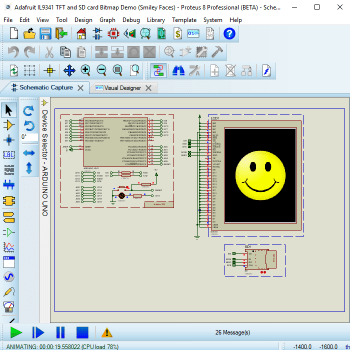
\includegraphics[width=0.3\paperwidth]{images/schematic}
        \caption{Tarjeta Arduino en Proteus}\footnotesize
        Fuente: \textit{Arduino Simulation Software - Processor, Shields and
        Peripherals} \cite{labcenter-electronics-2022}, bajo uso justo.
    \end{figure}

    \subsection{Instalar la Biblioteca de Arduino}

    En caso de ser necesario, se deberá instalar la biblioteca de Arduino
    para Proteus. Al finalizar con la simple instalación ya se podrá agregar
    la tarjeta Arduino desde la lista de dispositivos. Para mayor detalles,
    ir a \textit{How to Add Arduino Library in to Proteus 7 $\&$ 8}
    \cite{instructables-2018}.

    \subsection{Cálculo de la Resistencia del LED}

    El diodo LED se alimenta usualmente de una fuente directa de $3-5V$. La
    corriente y potencia del LED está especificada de acuerdo a cada diodo
    pero se sabe de antemano que algunos valores aproximados funcionan bien
    para un simple LED que se utilizará. Según \textit{Omni Calculator}
    \cite{szyk-2022} tenemos que conocer las siguientes variables:

    \begin{itemize}
        \item \textbf{Tipo de Circuito:} Serie o paralelo.
        \item \textbf{n:} Número de LED conectado.
        \item \textbf{V:} Fuente de voltaje.
        \item \textbf{$V_0$:} Caída de voltaje por cada LED\@.
        \item \textbf{$I_0$:} Corriente por LED\@.
    \end{itemize}

    Los valores estándar más comunes son configuración en serie; pilas,
    fuentes o baterías desde $1.5-12V$; voltaje de LED de $1.7-3.6V$ que
    depende del color del LED; y corrientes de $20-30mA$ \cite{szyk-2022}.

    \bigbreak

    Como bien sabemos por la ley de Ohm $R = \frac{V}{I}$ por lo que se
    deberá aplicar en el cálculo de la resistencia del LED\@.

    \bigbreak

    Para otros cálculos con configuración en serie tenemos que \cite{szyk-2022}:

    \begin{itemize}
        \item $R = \frac{V - n*V_0}{I_0}$
        \item $P_0 = V_0 * I_0$
        \item $P = n * V_0 * I_0$
        \item $P_r = I_0^2 * R$
    \end{itemize}

    \section{Procedimiento Experimental}

    El procedimiento consiste en la implementación en Arduino IDE y en Proteus.

    \subsection{Crear Programa Arduino}

    Primero hay que abrir un nuevo proyecto en Arduino IDE.

    \begin{figure}[H]
        \centering
        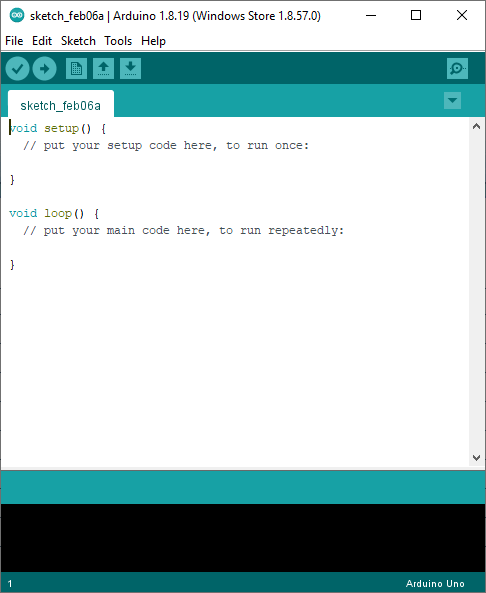
\includegraphics[width=0.3\paperwidth]{images/arduino-1}
        \caption{Programa inicial en Arduino IDE}
    \end{figure}

    Para actualizar el nombre del programa ir a File - Save As y seleccionar
    el directorio de destino y nombre del programa. En este caso, el nombre
    del programa es \say{activating-a-digital-output}.

    \bigbreak

    Se utilizará el siguiente programa sensillo para este laboratorio:

    \begin{lstlisting}[language=C, caption=Programa para activar una salida
    digital]
const int PIN = 12;

void setup()
{
    pinMode(PIN, OUTPUT);
}

void loop()
{
    digitalWrite(PIN, HIGH);
    delay(500);
    digitalWrite(PIN, LOW);
    delay(100);
}
    \end{lstlisting}

    \begin{figure}[H]
        \centering
        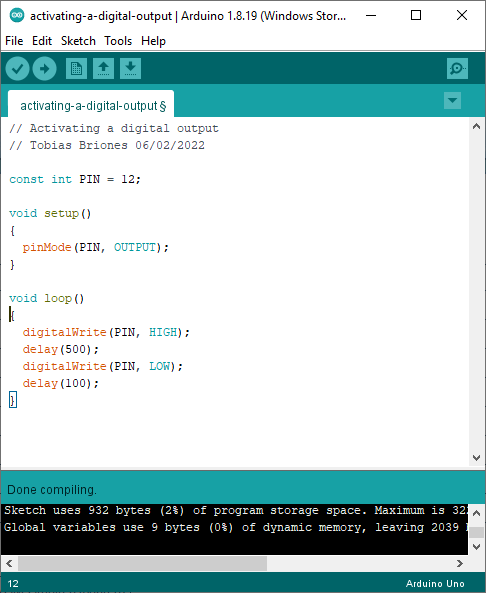
\includegraphics[width=0.3\paperwidth]{images/arduino-2}
        \caption{Programa final a correr}
    \end{figure}

    Para obtener el binario hexadecimal compilado del código fuente, ir a
    Sketch - Export compiled binary.
    Ahora, los archivos .hex compilados se encontrarán en el directorio donde
    del programa fue guardado.

    \subsection{Correr simulación en Proteus}

    Para correr la simulación se usará Proteus.

    \bigbreak

    Al abrir Proteus, ir a File - New Project dar un nombre al proyecto.

    \bigbreak

    Siguiente - Seleccionar \say{Crear un esquema del template selecciondado}
    con la opción \say{DEFAULT}.

    \bigbreak

    Siguiente - Seleccionar \say{No crear un layout PCB}.

    \bigbreak

    Siguiente - Seleccionar \say{Crear proyecto de firmware} con las opciones
    de Familia: ARDUINO, Controlador:
    Arduino Uno y Compilador: Arduino AVR (Proteus). Dejar seleccionado
    \say{Crear Archivos de Inicio Rápido}.

    \bigbreak

    Siguiente - Terminar.

    \begin{figure}[H]
        \centering
        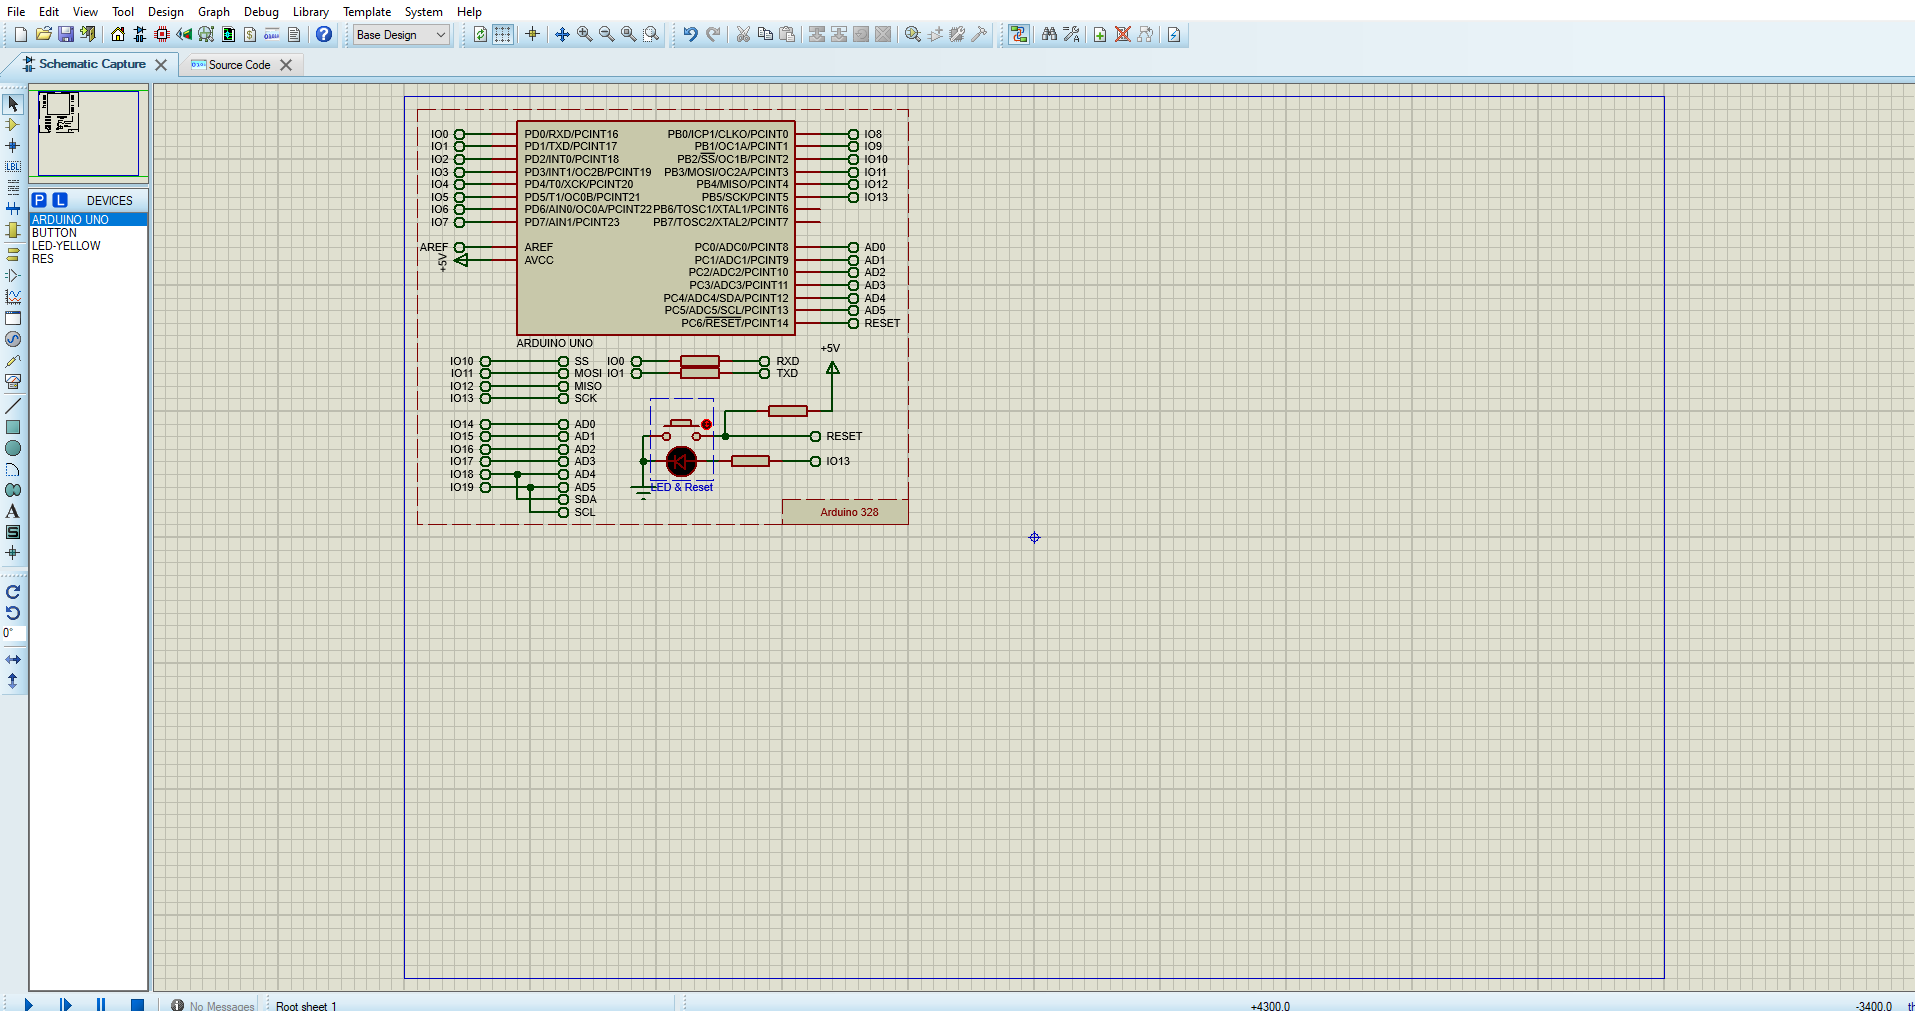
\includegraphics[width=0.5\paperwidth]{images/sim-1}
        \caption{Configuración inicial del Proteus con Arduino Uno}
    \end{figure}

    En el simulador se debe cargar el programa que se escribió. Dar click
    derecho a la tarjeta de Arduino e ir a
    Propiedades. En \say{Archivo de Programa} seleccionar el archivo binario
    que se compiló, que contiene el bootloader.
    En este caso, el archivo es \say{activating-a-digital-output.ino
    .with\_bootloader.standard.hex}.

    \bigbreak

    Calculando el valor de la resistencia tenemos que con valores estándar

    $$
    R_{LED} = \frac{5v}{20mA} = 100\Omega
    $$

    En caso de no ser exacto la resistencia en valor comercial se deberá
    redondear o aplicar otra configuración para obtener la resistencia
    equivalente.

    \begin{figure}[H]
        \centering
        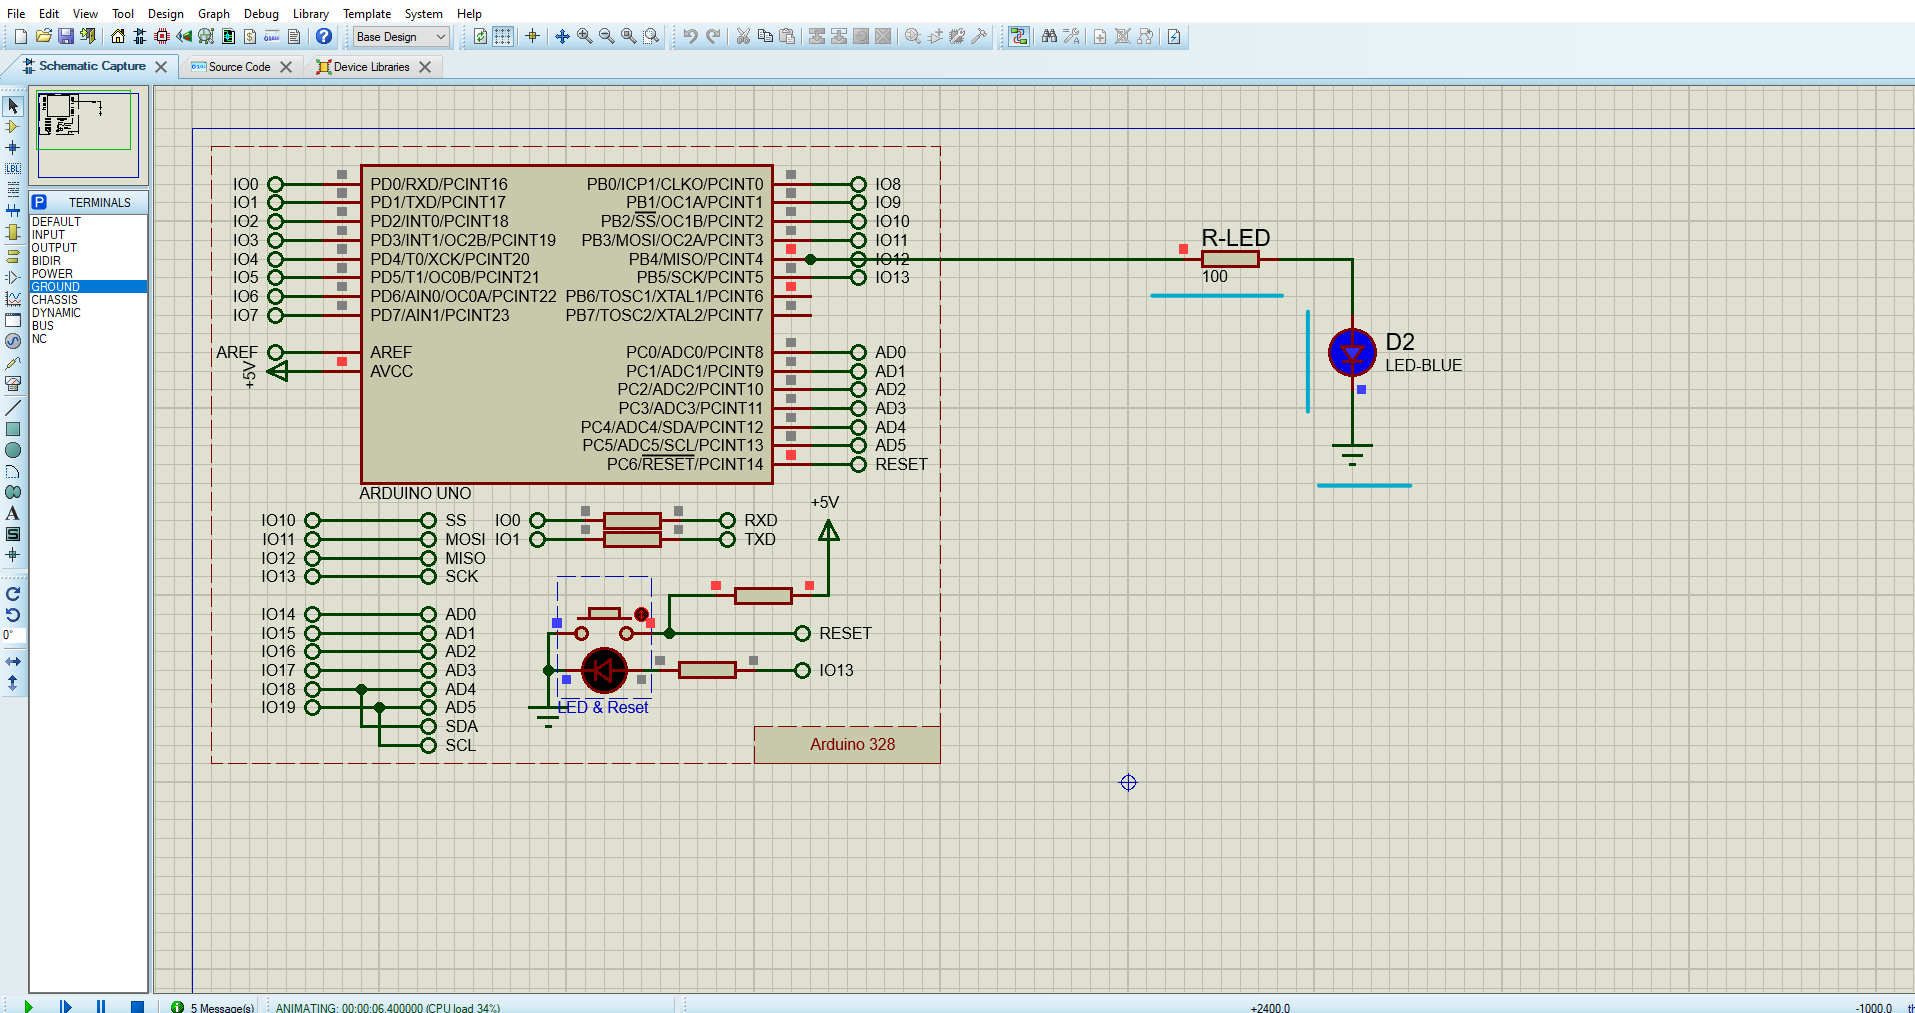
\includegraphics[width=0.5\paperwidth]{images/sim-2}
        \caption{Configuración del circuito final en Proteus}
    \end{figure}

    \section{Análisis de Resultados}

    Al correr satisfactoriamente el programa en Proteus, el LED $D2$ parpadea
    de acuerdo a las iteraciones establecidas en el programa. Tener en cuenta
    que la simulación puede correr más o menos rápido de acuerdo a la
    velocidad del simulador.

    \bigbreak

    La tarjeta Arduino emitió las señales digitales mediante el pin $12$ que
    se definió en el loop del programa.

    \section{Conclusión}

    Se desarrolló un programa en Arduino IDE que activa la señal del pin $12$
    del Arduino dado un intervalo establecido. Luego, se creó una simulación
    del circuito agregando un LED como carga a la salida $12$ del Arduino. Se
    calculó de antemano la resistencia del LED de forma que fuera de
    protección para este.

    \printbibliography

\end{document}
